%%=============================================================================
%% Performantietest
%%=============================================================================

\chapter{Performantie test}
\label{ch:performantietest}

In dit hoofdstuk worden de resultaten besproken van de uitgevoerde performantietests. De performantie van beide opstellingen werden getests Door gebruik te maken van 'time vagrant up' en 'time vagrant provision'. Hierdoor werd er op het einde van de installatie de tijd getoond die Vagrant nodig had om het commando uit te voeren. Beide commando's werden elk 15 keer uitgevoerd.

\subsection{CentOS 7.4}

\subsubsection{Performantie installatie}
Als eerste kan men hieronder de resultaten zien van 'time vagrant up' voor de CentOS-opstelling. Dit toont hoeveel tijd Vagrant nodig had om de CentOS opstelling te installeren vanaf nul tot een werkende webapplicatie.

%% plot
\begin{center}
	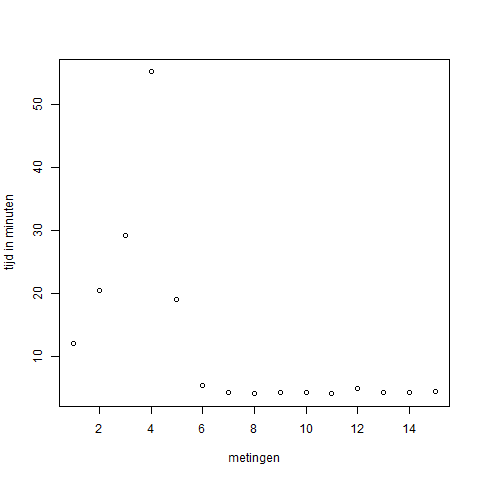
\includegraphics[scale=0.5]{img/centosplotfull.png}
\end{center}

%% gemiddelde
\[ \mu = 12.06457 \]
 
%% variantie
\[ \sigma^2 = 203.7204 \]

%% standaarddeviatie
\[ \sigma = 14.27307 \]

%% boxplot
\begin{center}
	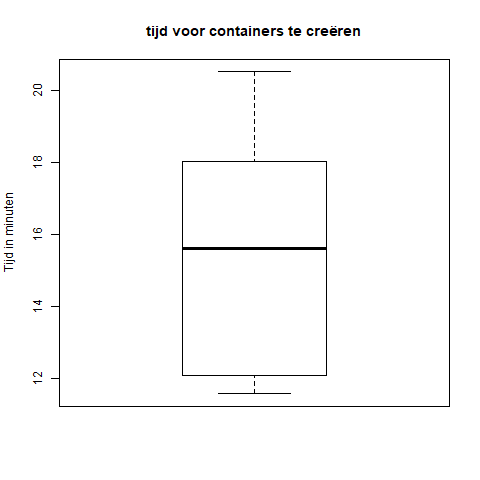
\includegraphics[scale=0.5]{img/centosboxplotfull.png}
\end{center}

De gemiddelde performatie-maat van de CentOS-opstelling is laag en vrijwel stabiel, met maar een paar uitschieters. De reden voor deze uitschieters komt omdat deze genomen zijn in een omgeving met een slechtere internetverbinding. Dit is dus de bottleneck bij deze opstelling en kan een grote impact hebben op de installatie, zoals te zien valt aan de hoge variatie en standaarddeviatie. Ondanks dit is de performantie van de CentOS-opstelling heel goed te noemen.

\subsubsection{Performantie applicatie}
Daarnaast kan men hier de resultaten zien van 'time vagrant provision'. Bij deze resultaten moet het Operating System niet meer geïnstalleerd worden, alleen nog maar de containers voor de applicatie.

%% plot
\begin{center}
	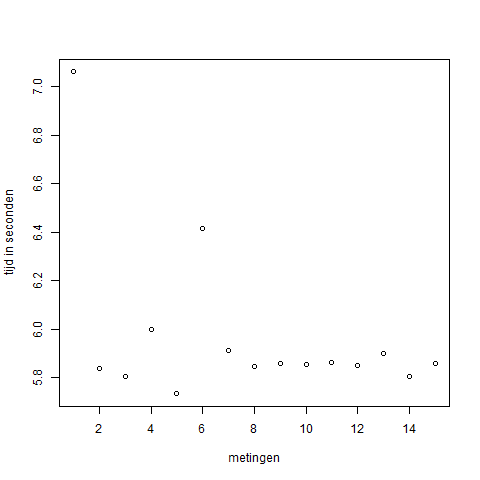
\includegraphics[scale=0.5]{img/centosplotprovision.png}
\end{center}

%% gemiddelde
\[ \mu = 5.972333 \]

%% variantie
\[ \sigma^2 = 0.1150491 \]

%% standaarddeviatie
\[ \sigma = 0.3391889 \]

%% boxplot
\begin{center}
	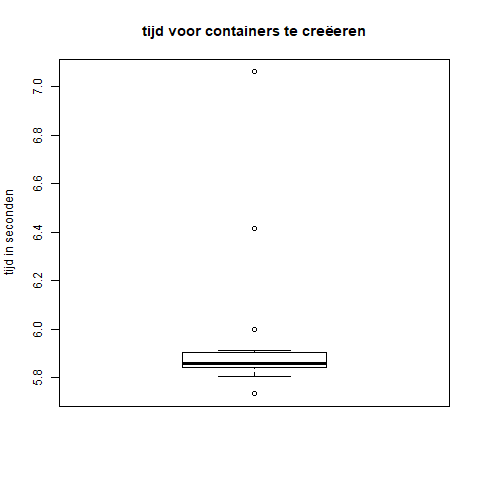
\includegraphics[scale=0.5]{img/centosboxplotprovision.png}
\end{center}

Ook het opstellen van alleen de container gaat vlot. Met een stabielere gemiddelde tijd en een kleinere variantie en standaarddeviatie. Doordat er geen tijd meer nodig was om de Docker Images te downloaden lagen de tijden veel lager.

\subsection{Windows Server 2016}
\subsubsection{Performantie installatie}
Vervolgens kan men ook de resultaten zien van 'time vagrant up' voor de Windows-opstelling.

%% plot

%% gemiddelde

%% variantie

%% standaarddeviatie

%% boxplot

De Windows opstelling brengt het er veel slechter vanaf dan de Linux opstelling. De gemiddelde tijd is immers 45 minuten en de variantie en standaarddeviatie liggen veel groter. Hier zijn er verschillende redenen voor:

\begin{itemize}[noitemsep]
	\item Installatie Windows OS
\end{itemize}

De installatie van het besturingssysteem zelf duurt langer omdat de Docker CE for Windows een GUI vereist. Met een Windows Server core zou de performantie al sterk verbeterd kunnen worden. Windows Server nano is helaas geen optie, omdat deze niet ondersteund wordt door Docker CE for Windows.

\begin{itemize}[noitemsep]
	\item Microsoft SQL server container
\end{itemize}

De MSSQL server container voor Windows is meer dan 10 keer zo groot als de Linux variant,  6GBs tegenover 479MBs. Hierdoor is het systeem een groot deel van zijn tijd bezig met downloaden van de Docker Image.

\subsubsection{Performantie applicatie}
Ten slotte kan men hieronder ook de resultaten zien van 'time vagrant provision' voor de Windows-opstelling van alleen de benodigde tijd om de containers te installeren.

%% plot

%% gemiddelde

%% variantie

%% standaarddeviatie

%% boxplot

Hier zijn de resultaten al iets meer genormaliseerd tegenover de CentOS-opstelling. Omdat de Windows-opstelling nu de extra bestanden voor de grafische interface of gigantische MSSQL image moet binnenhalen.